\section{Effective dynamics}

\subsection{Factorizable dynamics}

\begin{frame}{General solution}
    Factorizable unitary dynamics are of the form $\mcU_{t}=U_{1}^{t}\otimes U_{2}^{t}$.
    \begin{align*}
        \text{Since } \varrho=\rho_{A}\otimes\rho_{B} & & \Longrightarrow & &\rho\mapsto (1-p)U_{1}^{t}\rho_{A}(U_{1}^{t})^{\dag}+pU_{2}^{t}\rho_{B} (U_{2}^{t})^{\dag}.
    \end{align*}
    Expected values evolve as
    \begin{equation*}
            \expval{\pauli{i}(t)}=(1-p)\Tr[\pauli{i}U_{1}^{t}\rho_{A}(U_{1}^{t})^{\dag}]+p\Tr[\pauli{i}U_{2}^{t}\rho_{B}(U_{2}^{t})^{\dag}].
      \end{equation*}
\end{frame}


\begin{frame}{One example}
    \begin{columns}
        \begin{column}{0.5\textwidth}
            Let
            \begin{equation*}
                \rho=\frac{1}{2}\qty[\Id+\frac{4}{5\sqrt{2}}\qty(\frac{1}{2}\pauli{1}+\frac{1}{2}\pauli{2}+\pauli{3})],
            \end{equation*}
            and $\mcU_{t}=e^{-itH_{1}}\otimes e^{-itH_{2}}$ where
                \begin{align*}
                    H_{1}=\pauli{3} & & \text{and} & & H_{2}=\frac{\omega}{\sqrt{2}}(\pauli{1}-\pauli{2}).
                \end{align*}
            Solution:
            \begin{equation*}
                \expval{\pauli{3}(t)}=\expval{\pauli{3}(0)}+pr_{B}(\cos(2\omega t)-1).
            \end{equation*}
        \end{column}
        \begin{column}{0.5\textwidth}
            \begin{figure}[h!]
                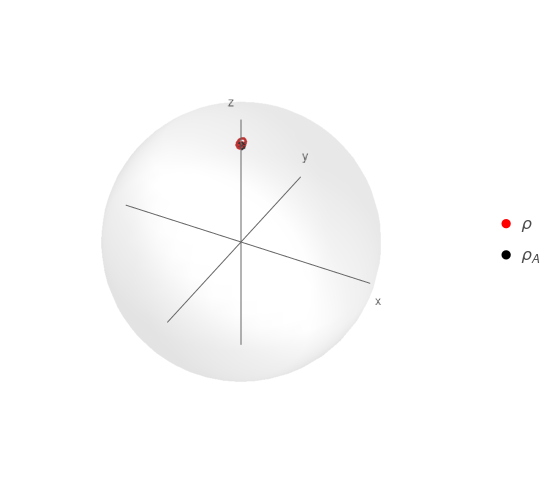
\includegraphics[width=0.7\columnwidth]{figures/U1xU2_H1=(sz)_H2=15(sx-sy)_z=0.8_p=0.9_far.png}%
                \caption{Oscillations near no-error trajectory.\\ $r=0.8$ $p=0.1$ and $\omega=15$. }
            \end{figure}
        \end{column}
    \end{columns}
\end{frame}

\begin{frame}{Two less specific cases}
     $r_{A}\hat{r}_{\rho}$ and $r_{B}\hat{r}_{\rho}$ are the Bloch vectors of $\rho_{A}$ and $\rho_{B}$. $O_{i}$ is the rotation induced by $U_{i}$.
    \begin{columns}
        \begin{column}{0.5\textwidth}
            \begin{itemize}
                \item If $U_{1}=\Id$ then:
                \begin{equation*}
                    r\hat{r}_{\rho}\mapsto r\hat{r}_{\rho}+p(O_{2}(r_{B}\hat{r}_{\rho})-r_{B}\hat{r}_{\rho}).
                \end{equation*}
            \end{itemize}
            \begin{figure}[h!]
                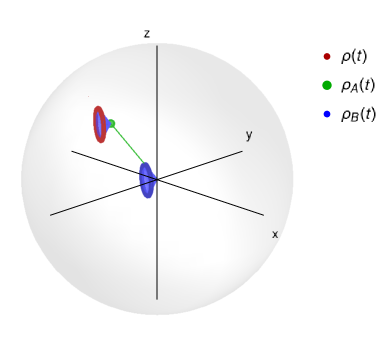
\includegraphics[width=0.6\columnwidth]{figures/U1xU2_H1=Id_H2=sz_z=0.8_p=0.6_sequence.png}%
                \caption{Oscillations near no-error trajectory.\\ $r=0.8$ $p=0.9$ and $\omega=15$. }
            \end{figure}
        \end{column}
        \begin{column}{0.5\textwidth}
            \begin{itemize}
                \item If $U_{2}=\Id$ then:
                \begin{equation*}
                    r\hat{r}_{\rho}\mapsto O_{1}(r\hat{r}_{\rho}-pr_{B}\hat{r}_{\rho})+pr_{B}\hat{r}_{\rho}.
                \end{equation*}
            \end{itemize}
            \begin{figure}[h!]
                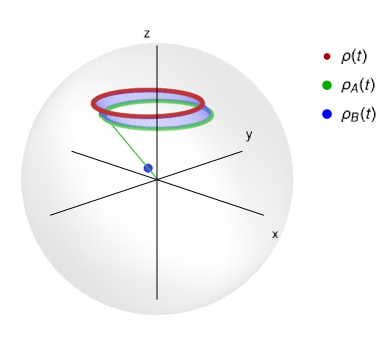
\includegraphics[width=0.6\columnwidth]{figures/U1xU2_H1=sz_H2=Id_z=0.8_p=0.7_sequence.png}%
                \caption{Oscillations near no-error trajectory.\\ $r=0.8$ $p=0.1$ and $\omega=15$. }
            \end{figure}
        \end{column}
    \end{columns}
\end{frame}


\subsection{SWAP gate}

\begin{frame}{Effective SWAP}
    \begin{columns}
        \begin{column}{0.5\textwidth}
            Effective state before and after:
            \begin{align*}
                \rho(0)&=(1-p)\rho_{A}+p\rho_{B},\\
                \rho(t=1)&=p\rho_{A}+(1-p)\rho_{B}.
                \end{align*}
                Contraction!:
                \begin{equation*}
                    \kappa_{t}=\frac{r_{\rho(1)}}{r_{\rho(0)}}.
                  \end{equation*}
                  Non linear depolarizing channel:
                  \begin{equation*}
                      \boxed{\rho\mapsto\kappa_{t}^{\rho}\rho+(1-\kappa_{t}^{\rho})\frac{1}{2}\Id}
                    \end{equation*}
        \end{column}
        \begin{column}{0.5\textwidth}
            \begin{figure}[h!]
                \centering
                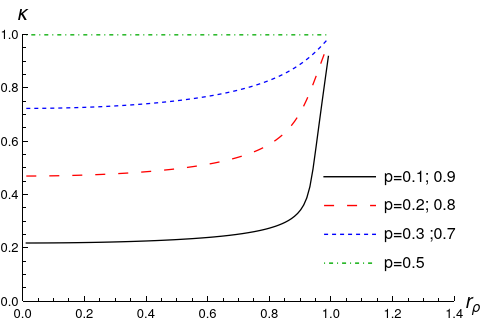
\includegraphics[width=0.9\linewidth]{figures/ContractionFactorSWAP_2D_r0to1_legend.png}
                \caption{Depolarizing coefficient as a function of $r_{\rho(0)}$ for different values of $p$.}
                \label{fig:SWAPFactor2D}
              \end{figure}
        \end{column}
    \end{columns}
\end{frame}


\begin{frame}{Effect on the Bloch sphere}
    \begin{figure}[h!]
        \centering
        \begin{subfigure}{0.32\textwidth}
            \centering
            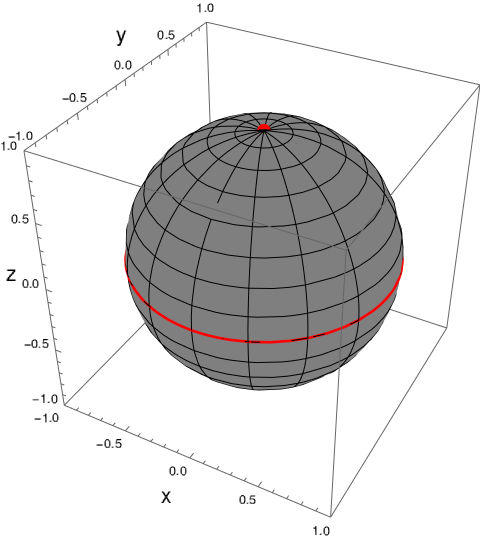
\includegraphics[width=0.9\linewidth]{figures/sphere_swapcontraction_t=0.0_z=0.9_p=0.9.png}
            \caption{$t=0.0$}
        \end{subfigure}%
        \begin{subfigure}{0.32\textwidth}
            \centering
            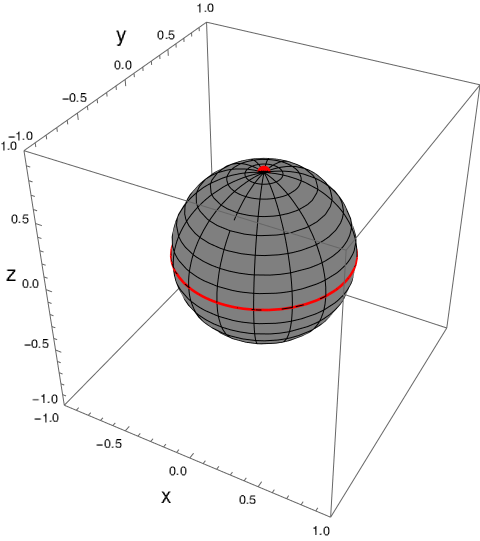
\includegraphics[width=0.9\linewidth]{figures/sphere_swapcontraction_t=0.5_z=0.9_p=0.9.png}
            \caption{$t=0.5$}
        \end{subfigure}
        \begin{subfigure}{0.32\textwidth}
            \centering
            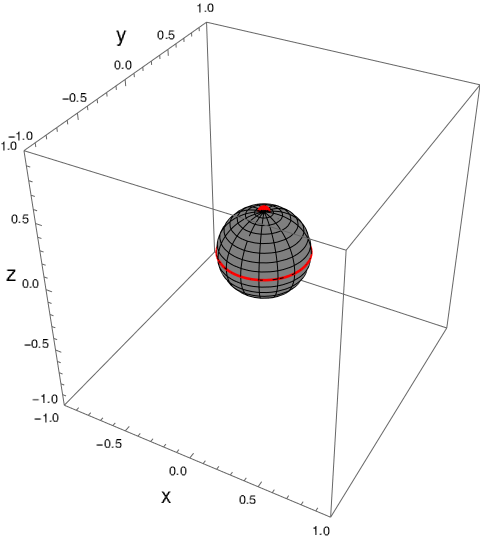
\includegraphics[width=0.9\linewidth]{figures/sphere_swapcontraction_t=1.0_z=0.9_p=0.9.png}
            \caption{$t=1.$}
        \end{subfigure}
        \caption{Effect on the Bloch sphere. $r=0.9$, $p=0.1$. $r(t)\leq r(0) \forall t$ since $\Gamma_{t}$ not reversible.}
    \end{figure}
\end{frame}

\subsection{CNOT gate}

\begin{frame}{Effective CNOT}
    We study
    \begin{equation*}
        \rho(t)=\CG{\cnot \mcA_{\mcC}^{max}[\rho(0)](\cnot)^{\dag}}
    \end{equation*}
    Initial efective state is
    \begin{equation*}
        \rho(0)=(1-p)\rho_{A}+p\rho_{B}.
    \end{equation*}
    Final efective state is
    \begin{align*}
        \rho(t=1)=&\frac{1}{2}[(1-p)(\rho(0)+\sigma_{3}\rho_{A}\sigma_{3}+\Tr{\sigma_{1}\rho_{B}}[\rho_{A}-\sigma_{3}\rho_{A}\sigma_{3}])\\
        &+p(\rho(0)+\sigma_{1}\rho_{B}\sigma_{1}+\Tr{\sigma_{3}\rho_{A}}[\rho_{B}-\sigma_{1}\rho_{B}\sigma_{1}])]
    \end{align*}.
\end{frame}

\begin{frame}{Phase flip channel}
    \begin{columns}
        \begin{column}{0.5\textwidth}
            Let's suppose $p=0$. The evolved effective state:
            \begin{equation*}
              \rho(t=1)=\frac{1}{2}\rho(0)+\frac{1}{2}\pauli{3}\rho(0)\pauli{3}.
            \end{equation*}
            This is a phase flip channel!
        \end{column}
        \begin{column}{0.5\textwidth}
            \begin{figure}[h!]
                \centering
                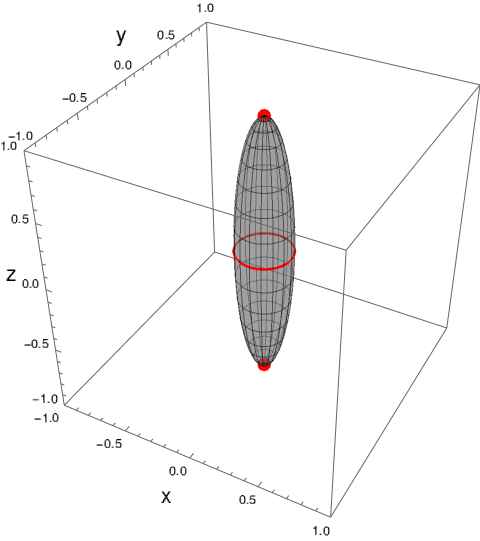
\includegraphics[width=0.7\linewidth]{figures/sphere_PF_t=1.0_z=0.8_p=0.6.png}
                \caption{Phase flip map}
                \label{fig:SWAPFactor2D}
              \end{figure}
        \end{column}
    \end{columns}
\end{frame}

\begin{frame}{Bit flip channel}
    \begin{columns}
        \begin{column}{0.5\textwidth}
            Let's suppose $p=1$. The evolved effective state:
            \begin{equation*}
              \rho(t=1)=\frac{1}{2}\rho(0)+\frac{1}{2}\pauli{1}\rho(0)\pauli{1}.
            \end{equation*}
        
            This is a bit flip channel!
        \end{column}
        \begin{column}{0.5\textwidth}
            \begin{figure}[h!]
                \centering
                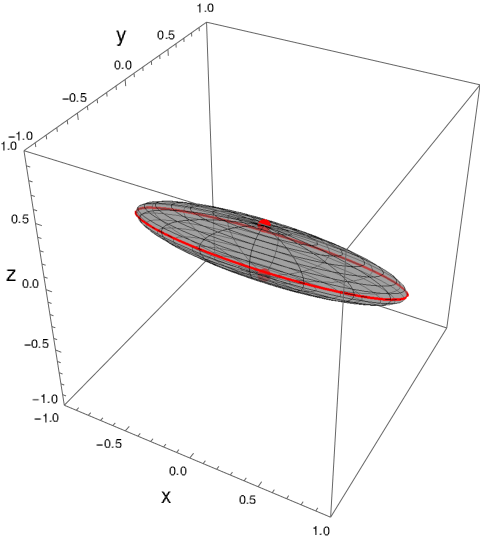
\includegraphics[width=0.7\linewidth]{figures/sphere_BitF_t=1.0_z=0.8_p=0.6.png}
                \caption{Bit flip map}
                \label{fig:SWAPFactor2D}
              \end{figure}
        \end{column}
    \end{columns}
\end{frame}


\begin{frame}{Effective CNOT}
    Back to our expression:
    \begin{align*}
        \rho(t=1)=&\frac{1}{2}\rho(0)\\
        &+\frac{(1-p)}{2}\qty[\expval{\pauli{1}}_{\rho_{B}}\rho_{A}+(1-\expval{\pauli{1}}_{\rho_{B}})\pauli{3}\rho_{A}\pauli{3}]\\
        &+\frac{p}{2}\qty[\expval{\pauli{3}}_{\rho_{A}}\rho_{A}+(1-\expval{\pauli{3}}_{\rho_{A}})\pauli{1}\rho_{B}\pauli{1}].
    \end{align*}
    Mix of a non linear bit flip channel and a non linear phase flip channel
\end{frame}

\begin{frame}{Almost a phase flip}
    \begin{figure}[h!]
        \centering
        \begin{subfigure}{0.32\textwidth}
            \centering
            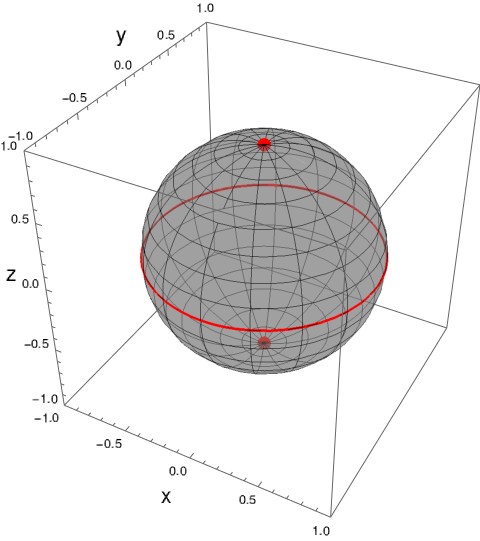
\includegraphics[width=0.9\linewidth]{figures/sphere_CNOT_t=0.0_z=0.8_p=0.95.png}
            \caption{$t=0.0$}
        \end{subfigure}%
        \begin{subfigure}{0.32\textwidth}
            \centering
            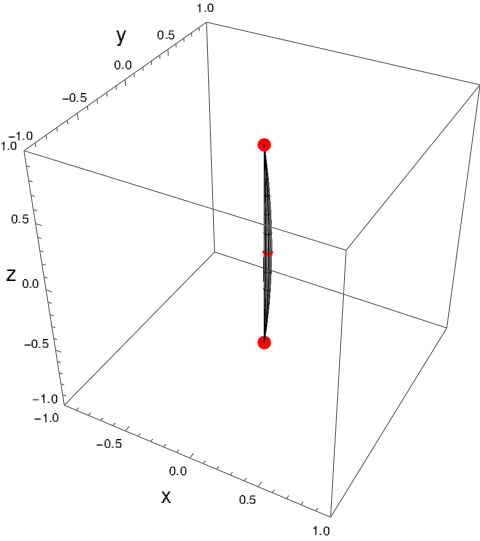
\includegraphics[width=0.9\linewidth]{figures/sphere_CNOT_t=1.0_z=0.8_p=0.95.png}
            \caption{$t=1.0$}
        \end{subfigure}
        \caption{Effect on the Bloch sphere. $r=0.8$, $p=0.05$.}
    \end{figure}
\end{frame}

\begin{frame}{Almost a bit flip}
    \begin{figure}[h!]
        \centering
        \begin{subfigure}{0.32\textwidth}
            \centering
            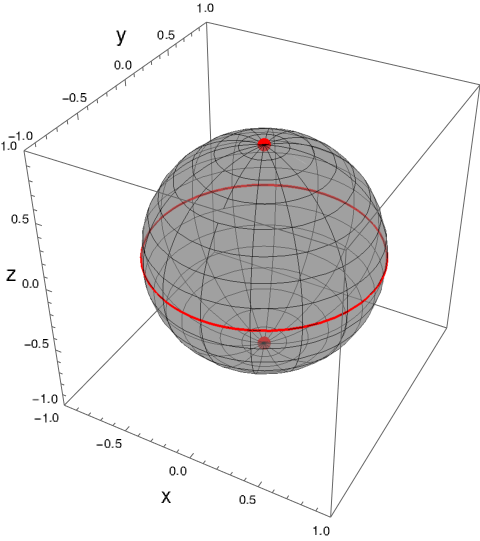
\includegraphics[width=0.9\linewidth]{figures/sphere_CNOT_t=0.0_z=0.8_p=0.05.png}
            \caption{$t=0.0$}
        \end{subfigure}%
        \begin{subfigure}{0.32\textwidth}
            \centering
            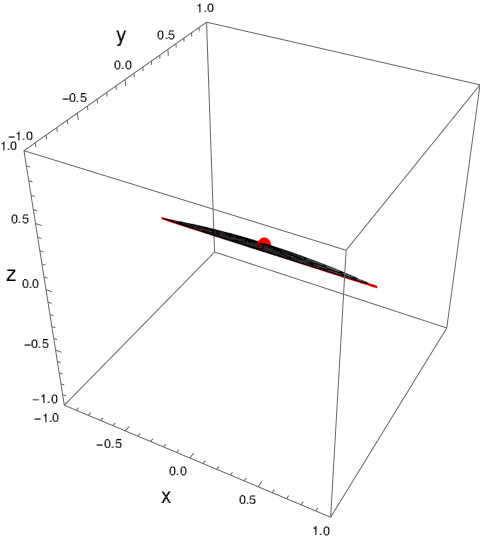
\includegraphics[width=0.9\linewidth]{figures/sphere_CNOT_t=1.0_z=0.8_p=0.05.png}
            \caption{$t=1.0$}
        \end{subfigure}
        \caption{Effect on the Bloch sphere. $r=0.8$, $p=0.95$.}
    \end{figure}
\end{frame}

\begin{frame}{Effective CNOT on the Bloch sphere}
    \begin{figure}[h!]
        \centering
        \begin{subfigure}{0.32\textwidth}
            \centering
            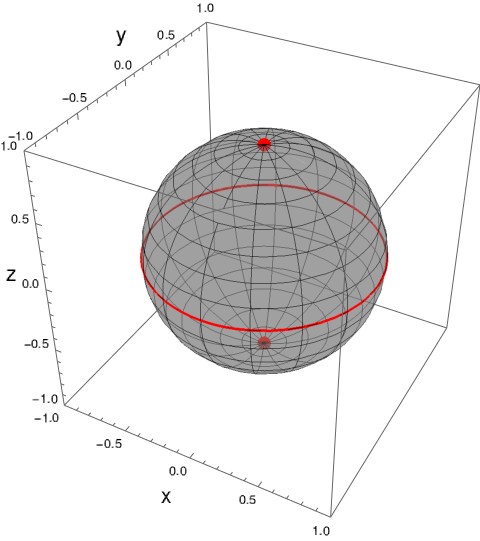
\includegraphics[width=0.9\linewidth]{figures/sphere_CNOT_t=0.0_z=0.8_p=0.6.png}
            \caption{$t=0.0$}
        \end{subfigure}%
        \begin{subfigure}{0.32\textwidth}
            \centering
            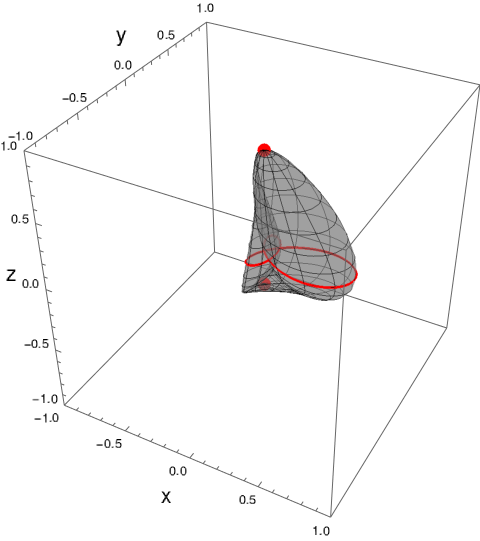
\includegraphics[width=0.9\linewidth]{figures/sphere_CNOT_t=1.0_z=0.8_p=0.6.png}
            \caption{$t=1.0$}
        \end{subfigure}
        \caption{Effect on the Bloch sphere. $r=0.8$, $p=0.4$.}
    \end{figure}
\end{frame}

\subsection{Current work: an Ising model}

\begin{frame}{Ising Model}
    We consider the following hamiltonian:
    \begin{align*}
        H=J\sigma_{z}\otimes\sigma_{z} && \Rightarrow && \mcU_{t}=\Id \cos{tJ} + i\sigma_{z}\otimes\sigma_{z}\sin{tJ}
    \end{align*}
    The evolved effective state looks like
    \begin{align*}
        \mcC{\varrho_{max}(t)}=&\rho(0)\cos^{2}{Jt}+\sigma_{3}\rho(0)\sigma_{3}\sin^{2}{Jt}\\
        &-i\frac{\lambda_{3}}{\lambda}\sin{Jt}\cos{Jt}[\sigma_{3},p\tanh((1-p)\lambda)\rho_{A}+(1-p)\tanh(p\lambda)\rho_{B}]
    \end{align*}
    Two important terms arise: the first is linear and independent of the coarse graining parameters, and the second one carries the non-linearity of the evolution, as it includes the Lagrange variable $\lambda$.
\end{frame}